\documentclass{paper}
\usepackage{float}
\usepackage{graphicx}
\usepackage{hyperref}
\usepackage{amsthm}
\usepackage{amsmath}
\usepackage{amsfonts}
\usepackage[style=authoryear,
    bibstyle=authoryear,
    backend=biber,
    natbib=true,
    maxnames=99,
    maxcitenames=2,
    uniquelist=minyear,
    giveninits=true,
    uniquename=mininit
]{biblatex}

\addbibresource{bibliography.bib}

\title{FPGA användningar inom post-kvant kryptografi}
\author{Viktor Horsmanheimo}
\date{\today}

\newtheorem{definition}{Definition}
\newcommand{\bR}{\mathbb{R}}
\newcommand{\bZ}{\mathbb{Z}}

\begin{document}
\maketitle

Kryptografiska system är ofta implementerade inom mjukvara, men under de
senaste decennierna har \textit{Field Programmable Gate Arrays} (FPGA) blivit
alltmer populära inom kryptografi. FPGAn är omprogrammerbar hårdvara som
använder sig av booleska funktioners egenskaper. Där man kan representera vilken
som helst funktion med hjälp av en sannings tabell, FPGAn implementerar dessa
tabeller i så kallade \textit{uppslags tabeller}. Då den behöver omprogrameras
ändrar man på värden i tabellerna.

Orsaken till att FPGAn har blivit populära är bland annat att i en mjukvaro
implementation av kryptografiska system så existerar det flera attack
vektorer, till exempel operativ systemet. Processorn är även en attack
vektor. Detta insåg man med Spectre, som utnyttjade processorns spekulativa
gren förutsägelse. Vi kan använda oss av FPGAn för att separera krypterings
systemet, vilket minimerar attack vektorerna. Man kan skapa ett system, där
mjukvaran aldrig kan komma åt de kryptografiska nycklarna.
% TODO

År 1994 uppfann Peter Shor en algoritm, då vi utvecklar en tillräckligt bra kvant dator
kommer NP-svåra problem bli lösbara till exempel diskreta logaritm problemet.
Våra nuvarande kryptografiska metoder använder sig av dessa svåra problem för
att hållas säkra, detta betyder att vi i framtiden behöver nya metoder. Det
finns flera olika problem som tros vara svåra även för kvantdatorer.
Problem baserade på gitter som \textit{Lärande Med Fel} (LMF), samt avkodning av
\textit{fel korrigerande koder} är exempel av problem som tros vara NP-svåra;
essen kommer dock att fokusera på gitter baserade problem.

\begin{definition}
    Givet en basis $B = \{v_1, \ldots, v_k\} \in \bR^n$ av lineärt
    oberoende vektorer. Gittret L är definierat på följande sätt.

    \[L = \left\{ \sum_{i=1}^n a_i v_i | a_i \in \bZ \right\}\]

\end{definition}

Inom gitter finns det olika problem som tros vara svåra för kvant datorer.
\textit{Kortaste vektor problemet} (KVP) är ett av problemen man tror är NP-svåra.

Låt $\gamma \in \bR_+$, vi definierar kortaste vektorn inom $L$ att vara

\[\lambda (L) = \min_{y \in L} ||y||\]

var $||.||$ är normala definitionen för längder inom $\bR^n$ där $||x|| =
\sqrt{\sum_{i = 1}^n x_i^2}$, var $x = (x_1, \ldots, x_n)$.


Kortaste vektor problemet är att hitta $x \in L$ så att $||x|| \leq \gamma
\lambda (L)$. LLL algoritmen klarar av att lösa KVP inom polynomisk tid för
$\gamma \geq (\frac{4}{2})^{\frac{n}{2}}$, vi måste alltså välja $\gamma$ att
vara mindre än det.

\begin{definition}
    Lärande med fel är definierat på följande sätt: låt
    \begin{itemize}
        \item $s \in \bZ^n_q$. Låt $A_{s,\chi}$ vara en sannolikhets fördelning
            över $\bZ^n_q \times \bZ_q$.
        \item Välj $m$ vektorer för $a \in \bZ^n_q$
        \item $e \in \bZ_q$ samplat från $\chi$
        \item Räkna $b = a \cdot s + e \mod q$

        \item Utmatning $(a,b)$
    \end{itemize}
\end{definition}

I 2005 visade Oded Regev att detta var ett svårt problem, han visade att om man
skulle kunna lösa LMF i polynomisk tid så kan man även lösa KVP i polynomisk
tid \citep{regev05}.

Sök problemet inom LMF är att hitta $s \in \bZ^n_q$ given en godtycklig mängd
prov från $A_{s, \chi}$.

LMF kryptosystemet fungerar på följande sätt \citep{FPGA_post_quantum}:

Låt $t = \lfloor \frac{q}{2} \rfloor$
\begin{itemize}
    \item \textbf{Nyckel generation:} vi väljer en hemlig nyckel
        $s \in \bZ^n_q$, en vektor $a \in \bZ^n_q$ och ett fel $e \leftarrow
        \chi$. Räkna $b = a \cdot t + e$, allmänna nyckeln blir $(a,b)$.

    \item \textbf{Kryptering:} låt ett meddelande vara $m \in \{0,1\}$, $r_0,
        r_1, r_2 \leftarrow \chi$, chiffertexten blir $\{c_0, c_1\}$

        \[
            \begin{cases}
                c_0 = b \cdot r_0 + r_2 + t m\\
                c_1 = a \cdot r_0 + r_1
            \end{cases}
        \]

    \item \textbf{Dekryptering:} man räknar
        \[m = \lceil (c_0 - c_1 \cdot s) / t \rfloor \]
        Där $\lceil \rfloor$ avser avrundning till närmaste heltal.
\end{itemize}

Som vi ser ovan så har vi mycket vektor multiplikation, ett klassiskt sätt att
minska komplexitet är att beakta vektorerna som polynom. Därför används ringen
$R_q = \bZ_q [X] / \langle X^n + 1 \rangle$ istället för $\bZ^n_q$. Vektorn
$a = (a_0, \ldots, a_{n-1}) \in \bZ^n_q$ kan ses som polynomet
$P(x) = a_0 + \ldots + a_{n-1} x^{n-1} + x^n$ var $x$ är primitiva roten av
$x$.

\begin{figure}[H]
    \centering
    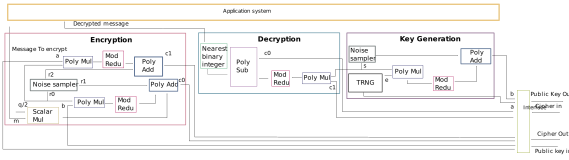
\includegraphics[scale=0.15]{high_level_impl.png}
    \caption{Hög nivå implementering av LMF \citep{FPGA_post_quantum}}
    \label{fig:high_level_impl}
\end{figure}

I Figur \ref{fig:high_level_impl} ser vi en hög nivå implementation av detta
kryptosystem, i denna esse kommer vi inte att gå in på hur \textit{True Random
Number Generator} fungerar samt \textit{Noise Samplern} fungerar. Vi har
försökt undvika dyra operationer som modulo då de tar väldigt många uppslags
tabeller.

\textit{Polynomisk addition/subtraktion} är implementerat med hjälp
av att göra operationen komponentvis och använder sig av villkorlig lagring
för att undvika modulo operationen.

\textit{Skalär multiplikation}, då vi räknar $t\cdot m$ väljer vi i princip
$t$ eller $0$ detta är möjligt för att $m$ är en $n$ bit vektor. På grund av
det kan vi kan igen använda oss av villkorlig lagring för att undvika
användning av modulo.

Låt $g = (c_0 - c_1 \cdot s)$, då vi räknar
\textit{skalär division till närmaste heltal} så kan vi använda oss av att
närmaste heltal kommer att vara $|g - t| < \frac{t}{2} \quad ? \quad 1 \quad :
\quad 0$. Detta är på grund av att $|g - t|$ räknar distansen mellan $g$ och
$t$, om resultatet är större än halva $t$ så är de långt från varandra och
kvotet kommer att vara 0. Å andra sidan om de är nära varandra så kommer
kvotet att vara 1.

\textit{Polynomisk multiplikation} är den komplexaste delen i vår design, vi
använder oss av \textit{Nummer Teoretiska Transformen} (NTT) för att göra
multiplikation snabbare. NTT är en generaliserad form av diskreta
fouriertransformen över ringen $R_q = \bZ_q[X] / \langle X^n + 1 \rangle$. NTT
definieras på följande sätt, låt $\omega$ vara $n$te enhetsroten för polynomet.

\[ X_i = \sum_{k=0}^{n-1}x_k \cdot \omega^{ik} \]

På normala sätt att multiplicera komponenterna har multiplikation en
komplexitet av $\mathcal{O}(n^2)$ men med NTT är komplexiteten
$\mathcal{O}(n\log n)$. För mera detaljer om hur NTT är implementerat, referera
till \citep{FPGA_post_quantum}.

\printbibliography

\end{document}
